\documentclass[a4paper, 12pt]{article}
\usepackage[a4paper,top=1.5cm, bottom=1.5cm, left=1cm, right=1cm]{geometry}
\usepackage{cmap}
\usepackage{mathtext}
\usepackage[T2A]{fontenc}
\usepackage[utf8]{inputenc}
\usepackage[english,russian]{babel}
\usepackage{multirow}
\usepackage{graphicx}
\usepackage{wrapfig}
\usepackage{tabularx}
\usepackage{float}
\usepackage{longtable}
\usepackage{hyperref}
\hypersetup{colorlinks=true,urlcolor=blue}
\usepackage[rgb]{xcolor}
\usepackage{amsmath,amsfonts,amssymb,amsthm,mathtools}
\usepackage{icomma}
\usepackage{euscript}
\usepackage{mathrsfs}
\usepackage{enumerate}
\usepackage{caption}
\usepackage{enumerate}
\mathtoolsset{showonlyrefs=true}
\usepackage{graphicx}
\usepackage{caption}
\usepackage{subcaption}
\usepackage{amsthm}
\usepackage[europeanresistors, americaninductors]{circuitikz}
\DeclareMathOperator{\sgn}{\mathop{sgn}}
\newcommand*{\hm}[1]{#1\nobreak\discretionary{}
	{\hbox{$\mathsurround=0pt #1$}}{}}

\newcommand{\framedtext}[1]{%
\par%
\noindent\fbox{%
    \parbox{\dimexpr\linewidth-2\fboxsep-2\fboxrule}{#1}%
}%
}

\title{\textbf{Изучение гальванометра{ (3.2.6)}}}
\author{Манро Эйден}
\date{}

\begin{document}

\maketitle

\newpage

\subsection*{Цель работы:}
изучение работы высокочувствительного зеркального гальванометра магнитоэлектрической системы в режимах измерения постоянного тока и электрического заряда.

\subsection*{В работе используются:}
зеркальный гальванометр с осветителем и шкалой, источник постоянного напряжения, делитель напряжения, магазин сопротивлений, эталонный конденсатор, вольтметр, переключатель, ключи,
линейка.

\section*{Экспериментальная установка}

\begin{wrapfigure}{l}{0.5\textwidth}
  \begin{center}
    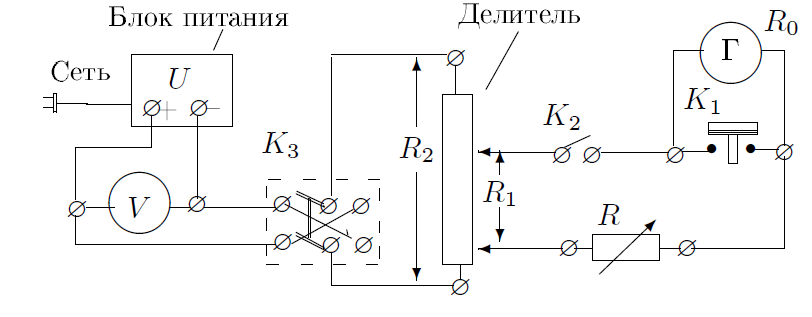
\includegraphics[width = 0.5\textwidth]{scheme_1.png}
  \end{center}
  \textbf{\caption{Схема установки для работы гальванометра в стационарном режиме}}
\end{wrapfigure}

Схема для исследования гальванометра в стационарном режиме
представлена на рис. 1. Постоянное напряжение $U$ снимается с блока
питания и измеряется вольтметром $V$. Ключ $K_3$ позволяет менять направление
тока через гальванометр $\Gamma$, делитель напряжения — менять
величину тока в широких пределах. Ключ $K_2$ служит для включения
гальванометра, кнопка $K_1$ — для его успокоения. Магазин сопротивлений
$R$ позволяет менять режим работы гальванометра от колебательного
до апериодического.

\begin{wrapfigure}{l}{0.5\textwidth}
  \begin{center}
    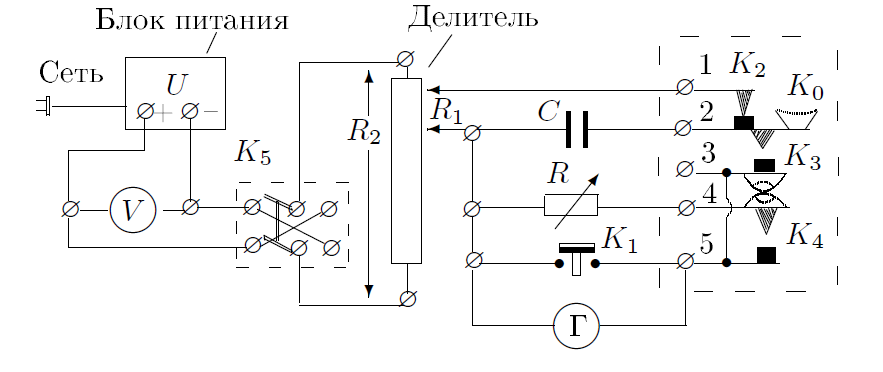
\includegraphics[width = 0.5\textwidth]{scheme_2.png}
  \end{center}
  \textbf{\caption{Схема установки для определения баллистической постоянной}}
\end{wrapfigure}

Для изучения работы гальванометра в режиме измерения заряда (в баллистическом режиме), используется схема, представленная на рис. 2.

Система ключей устроена так, что нормально ключ $K_2$ замкнут, а ключи $K_3$ и $K_4$ разомкнуты. При нажатии на кнопку $K_0$ сначала размыкается ключ $K_2$, затем замыкается $K_3$ и через некоторое время — $K_4$. При нормальном положении кнопки $K_0$ конденсатор $C$ заряжается до напряжения $U_C$ и получает заряд $q$.

При нажатии на ключ $K_0$ конденсатор отключается от источника постоянного напряжения (размыкается ключ $K_2$) и подключается к гальванометру (замыкается ключ $K_3$).

\begin{center}


\bigskip

\subsection*{Теоретическая справка}
\end{center}
\textit{Баллистический гальванометр} -- электроизмерительный прибор магнитоэлектрической системы, отличающийся высокой чувствительностью к току и сравнительно большим периодом свободных колебаний. \par
На помещённую в магнитное поле обтекаемую током рамку гальванометра действуют момент закрученной нити, момент магнитных сил и тормозящий момент (зависит от сил сопротивления воздуха и от вихревых токов). Учитывая все эти моменты, уравнение движения рамки принимает вид
\begin{center}
    $\ddot \varphi + 2 \gamma \dot \varphi + \omega_0^2\varphi = KI $,
\end{center}
где $\gamma$ -- коэффициент затухания подвижной системы гальванометра, $\omega_0$ -- собственная частота колебаний рамки

Динамическая постоянная гальванометра определяется при пропускании через рамку постоянного тока:
\begin{center}
    $C_I = \frac{I}{\varphi} = \frac{D}{BSN}$,
\end{center}
где $B$ - индукция магнитного поля в рамке, $S$ - площадь одного витка рамки, $D$ - модуль кручения нити. \par
При пропускании коротких импульсов тока через баллистический гальванометр начальная скорость движения рамки пропорциональна электрическому заряду, прошедшему через рамку за всё время импульса. Отношение баллистических постоянных в критическом и свободном режимах равно $e$.

\section*{Формулы}

\begin{align*}
    C_I &= \frac{2aI}{x} & S_I &= \frac{1}{C_I} \\
    \Theta &= \ln{\frac{x_n}{x_{n+1}}} & C^{\text{кр}}_q &= 2a \frac{R_1}{R_2} \frac{CU_0}{x^{cr}_{max}} \\
    \tau &= CR_0
\end{align*}


\section*{Ход работы}

\begin{figure}[H]
    \captionsetup{position=above, skip=2pt}
    \centering
    \caption{Зависимость $I(x)$}
    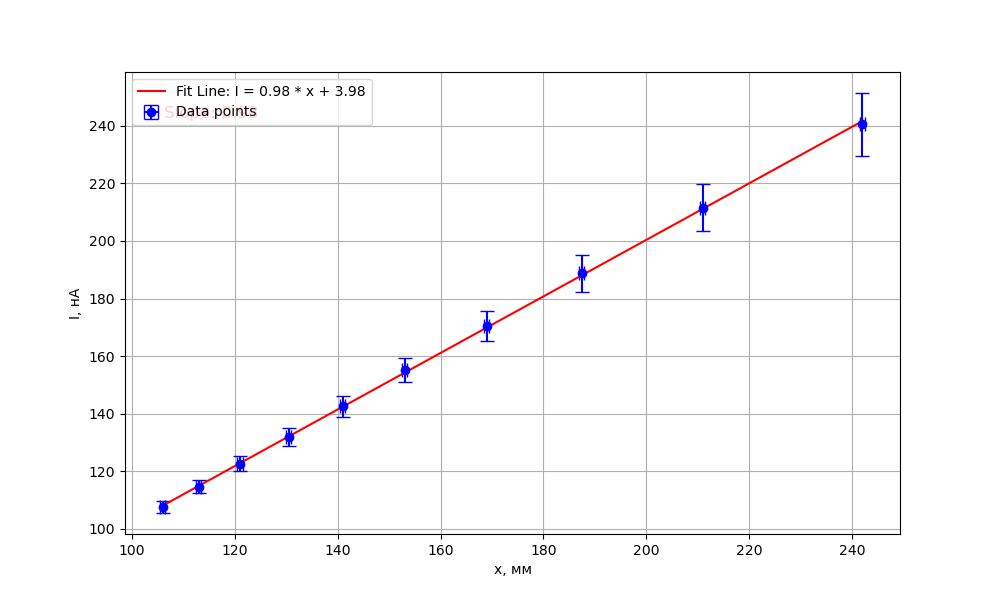
\includegraphics[width=\textwidth]{I_x/graphs/combined_graph.png}
\end{figure}

\newpage

Динамическая постоянная:

\begin{equation}
    C_I = (2612.28 \pm 130.85) \; \text{нА}
\end{equation}


Чувствительность гальванометра к току:

\begin{equation}
    S_I =( 0.38 \pm 0.02) \cdot 10^{-3} {\text{нA}}^{-1}
\end{equation}


Логарифмический декремент затухания:

\begin{equation}
    \Theta_0  = (192.12 \pm 3.28) \cdot 10^{-3}
\end{equation}

\begin{figure}[H]
    \captionsetup{position=above, skip=2pt}
    \centering
    \caption{Зависимость $(R+R_0)^2$}
    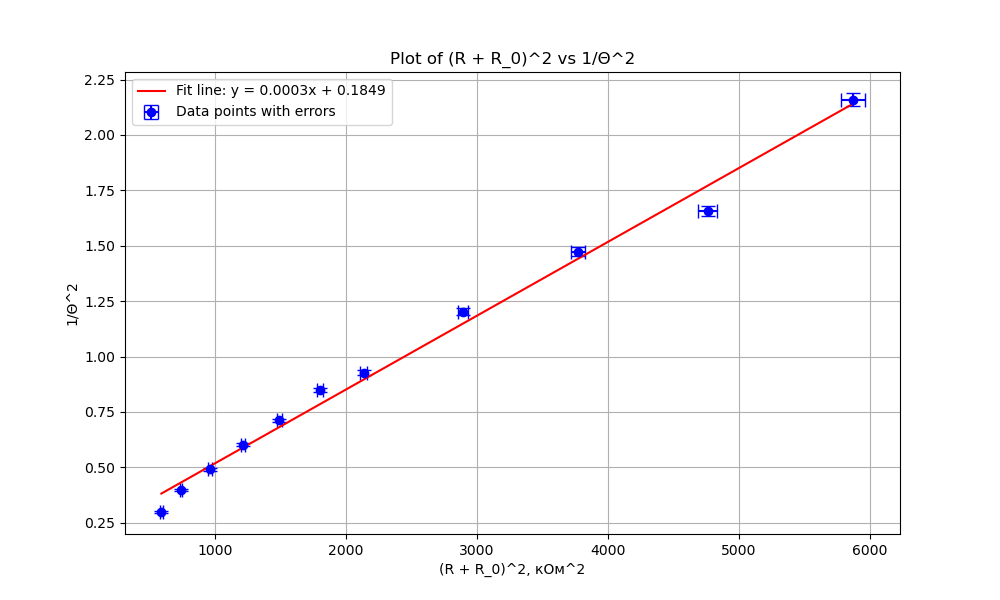
\includegraphics[width=\textwidth]{theta_R/graph.png}
\end{figure}


Критическое сопротивление, отпределенное по формуле:

\begin{equation}
    R_{\text{кр}} = (6813.22 \pm 94.98) \; \text{Ом}
\end{equation}

Критическое сопротивление, отпределенное по подбором:

\begin{equation}
    R_{\text{кр}} = (7600 \pm 100) \; \text{Ом}
\end{equation}

Баллистическая постоянная в критическом режиме:

\begin{equation}
    C^{\text{кр}}_q  = (1807.76 \pm 27.90) \; \text{нКл}
\end{equation}

Время релаксации:

\begin{equation}
    \tau =  (1.1 \pm 0.02) \; \text{мс}
\end{equation}


Период свободных колебаний гальванометра

\begin{equation}
    T_0 = (3.52 \pm 0.02) \; \text{с}
\end{equation}

Время релаксации крайне маленькое в сравнении с периодом свободных колебаний.


\section*{Вывод}

Убедились в линейности зависимости тока через гальванометр $I$ от его отклонения $x$.
Период колебаний подвижной системы получился сравнительно большим, а чувствуительность к току высокой, что соответсвует теоретическому описанию.

\end{document}
